\documentclass[10pt,conference,compsocconf]{IEEEtran}

\usepackage{hyperref}
\usepackage{graphicx}	% For figure environment


\begin{document}
\title{Digital 3D Geometry Processing - Project\\
Deliverable 1}

\author{
  Rapha\"{e}l Steinmann\\
	Thomas Batschelet\\
	Alain Milliet\\
  \textit{Department of Computer Science, EPFL, Switzerland}
}

\maketitle


\section{Goals}
\label{sec:goals}
Given the geralt mesh we want to create a lamp that is interesting to see, implement and that gives interesting lightning effects. Therefore we found the concept of water-like mesh. It would mean that we simulate a liquid falling on the mesh and what sort of bounce it would do on it (see figure~\ref{fig:water}).
 
\begin{figure}[tbp]
	\centering
	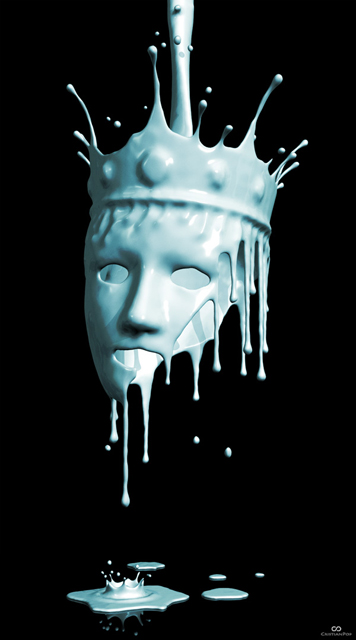
\includegraphics[width=\columnwidth]{liquid_mesh}
	\caption{Simulate water falling on a mesh}
	\vspace{-3mm}
	\label{fig:water}
\end{figure}

The implementation can be pretty challenging, so we prefer to give a plan 2 if we cannot find a way to make it. Plan 2 would be to apply artistic pattern on the mesh and disable some faces to create holes in it (like in the example~\ref{fig:bear})
 
\begin{figure}[tbp]
	\centering
	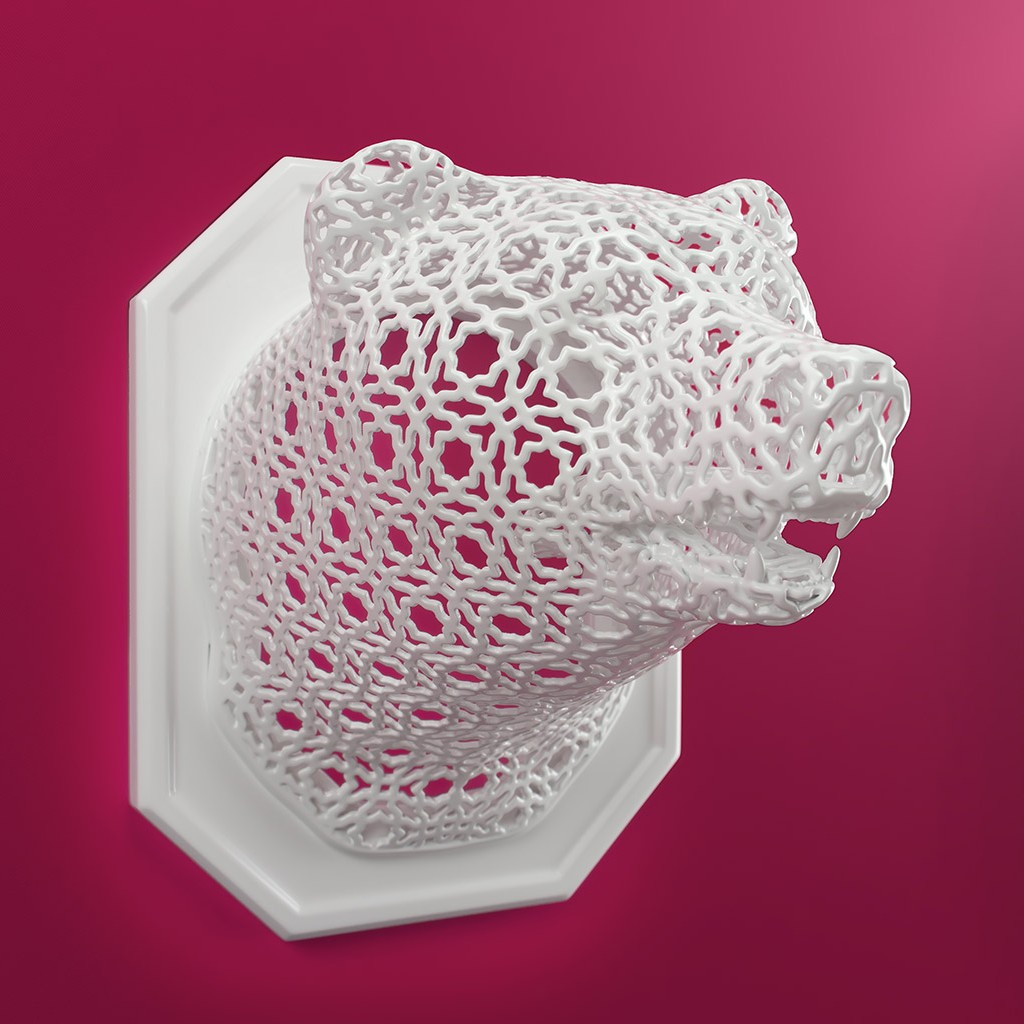
\includegraphics[width=\columnwidth]{3d-printed-lamps-animal-lace-bear}
	\caption{Pattern application on a bear-like mesh}
	\vspace{-3mm}
	\label{fig:bear}
\end{figure}

For both of this implementation we will need to have a really clean and smooth model at the beginning. See section ~\ref{sec:tools} for more details on what tools we will use to clean our mesh.


\section{Methods}
\label{sec:methods}
To reach our goals we will need to implement several methods. First of all we will have to smooth our mesh and make it as uniform as possible (vertex/face/edge-wise). For this matter we will use techniques we have seen during the course and labs (using curvature to smooth the object for example).\\
We will also need to implement new methods if we want to achieve a result that looks like figure~\ref{fig:water}. 
\textbf{TODO Maybe talk about http://matthias-mueller-fischer.ch/publications/posBasedDyn.pdf}

\section{Tools}
\label{sec:tools}
For this project we will use different existing tools to clean our mesh. We will first of all use meshlab to remove several default our mesh can contain (duplicate faces and vertices, zero area faces, unreferenced vertices, ...).\\\\
Then we will use netfabb to make a default repair of the mesh. The repair should fixe those different possible problems : 
\begin{enumerate}
\item Zero Holes: model will be manifold, without any gaps between faces and edges.
\item Zero Border Edges: a border edge is an edge on the side of a hole, or the edge side of a plane if another edge is it's missing.
\item Zero Invalid Orientations: In Netfabb, the direction of a face is shown in green if it points outward, red if it points inward. If you have red faces pointing out, that will be invalid orientation because it is inconsistent.
\item Positive Volume: All the green faces face out and the red face in, otherwise the printer will think that everything outside the model is material causing printer issues.
\item Closed Surfaces: A closed surface means that there are no holes or border edges.
\item Orientable Surface:All faces must be defined as in or out, with no stray edges or vertices.)
\end{enumerate}


\end{document}
